%%% -*-LaTeX-*-

\chapter{Introduction}

\setupuuchapterbib
%Digital computing is ubiquitous in any field of science.
%
In many domains of science where computers are used, a software developer needs to implement the solution to a mathematical problem, or to develop a mathematical algorithm in the machine.
%
Unfortunately, the developer cannot simply transcribe one-to-one the algorithm 'from the paper' to the computer.
%, using one of the many available programming languages.
%
%(e.g., Java, Python).
%
The main reason is the machine computes with finite resources, while in our ideal algorithm, we compute in real arithmetic, thus with infinite resources.
%
In mathematics, there are quantities, like for example $\pi$ or $\sqrt{2}$ or any other irrational number, with an infinite number of digits, and thus they cannot be represented \emph{exactly} using a finite representation.
%
These numbers have to be \emph{rounded} to fit the finite representation, and the gap between the real number and the rounded counterpart is named \emph{roundoff error}.

%
Computers store numbers in the form of a finite sequence of binary digits, which \emph{unavoidably} result in inaccurate computations.
%
The precision format (often called \emph{bit width} in the literature) is the length of the sequence used to represent numbers in the machine.
%
As a rule of thumb, the wider the precision format the more accurate are the computations.
%
At this point, a naive software developer might want to use a very wide bit width format to mimic real arithmetic. 
%
In other words, the inexperienced developer might decide to use a high-cost format, like for example 10000bits, as a proxy for real arithmetic.
%

There are several reasons why this approach does not solve our problem in practice.
%

First, computing using a finite precision format results in roundoff errors regardless of the bit width being used.
%
To put it simple, computing with 10000bits is not the same as computing with infinite bits.
%
Indeed, finite-precision arithmetics does not respect the rules of real arithmetic done with 'pen and paper'.
%
For example, the associativity law from real arithmetic fails in finite-precision where $(a*b)*c \ne a*(b*c)$.

Second, high-cost formats are very expensive in terms of resources which include, among the others, energy-consumption, execution time, and hardware dimensions~\cite{fppower, lutnet}. 
%
The usage of resources is critical on portable devices, like smart-phones or smart-watches, where the battery consumption is a primary concern.
%

Moreover, when dealing with chips with size in the order of $mm^{2}$, like micro-controllers, or where the available memory is very limited, in the order of the KB, it is unimaginable to compute using high-cost formats.
%

We have to live with the fact the arithmetic in computers is imprecise.
%
On the other hand, we cannot simply ignore the the roundoff error stemming from the use of finite-precision arithmetic, because it can have catastrophic consequences on the correct execution of the program.
%

For example, consider the program in Figure~\ref{fig:while}.
%
\begin{figure}[tb!]
	\begin{lstlisting}[frame=single, language=Python]
  n=0
  t=0
  while True:
    t = t + 1
    n = n + 0.1
	\end{lstlisting}
	\caption{A simple while loop with an imprecise accumulator showing the effect of roundoff errors.}\label{fig:while}
\end{figure}
%
After an execution time of 10 seconds, the value of the variable t is 231047636, while the value of the variable n is roughly 23104763.55.
%
Ideally, the value of n should be 23104763.6.
%
There is an absolute roundoff error of 0.45 in this program.
%
The reason behind such error is the decimal constant 0.1 is not exactly representable in binary (see Figure~\ref{fig:zeropointone} for a detailed explanation). 
%
At every iteration of the while loop, there is an absolute roundoff error of approximately 5.55e-18, stemming from the double-precision floating-point representation of the decimal 0.1. 
%

From an implementation perspective, a similar issue was the cause of the Patriot Missile Failure~\cite{patriot}.
%
In more details, during the Gulf War in 1991, an American Patriot Missile Defense battery failed to intercept an incoming missile.
%
The cause of the failure was the internal clock, in the Patriot battery, used to measure time in tenths of second.
%
This number was then multiplied by the decimal constant 0.1, which we know is not exactly representable, to produce the time in seconds.
%
The Patriot battery had been up and running for about 100 hours, and follow-up investigations showed the accumulated roundoff error corresponded to a travel time of 0.34 seconds for an incoming missile. 
%
In this amount of time, the incoming missile could travel for about half a mile.

In numerical analysis, the branch of rigorous mathematics concerning the analysis of numerical algorithms to implement the solutions to mathematical problems, we study how roundoff errors propagate through computations and what is their effect on the correct execution of a computer program. 

%

%Moreover, the \emph{single} and \emph{double} floating-point formats, nowadays a standard-de-facto for what concern arithmetic in computers, are not accurate enough for many applications which, among the others, include climate modeling~\cite{climate}, thermodynamic simulation~\cite{termodynamics}, fluid dynamics~\cite{fluiddynamics, statsfluiddynamics}, computational geometry applications~\cite{javaerror}, computational number theory~\cite{futurescience} and differential equations~\cite{differentialequations}.
%
%EXPAND ONE SENTENCE PER PAPER. KEEP ONLY 3. mATRIX MULTIPLICATION. POINT IN POLYGON (nasa PAPER). 
%cONTROLLERS.
%
%The gap between the ideal and the finite-precision computations is called roundoff error, and can have catastrophic consequences on the correct execution of a program.
%
%It is then critical, not only to be aware of the existence of this gap, but also to bound the arithmetic difference between the two programs.
%Numerical analysis is the branch of rigorous mathematics concerning the analysis of numerical algorithms used to implement the solutions to mathematical problems~\cite{higham2002accuracy}. 
%
\section{Computation Errors}
%

Finite-precision arithmetics, like floating-point, makes mathematic feasible in computer machines. 
%
Regardless of the base used for the representation (usually base 2 in the machine), not all the numbers can be exactly represented using a finite number of bits.
%
For example, periodic and irrational numbers, like $0.1$ or $\pi$, have to be rounded to fit the format of the representation. 
%
%The wider the format used for the representation, the smaller the gap between the real value and the value stored in the machine.
%
%In this thesis, we represent computed quantities with a hat (e.g., $\widehat{x}$) to distinguish from the real counter-part (e.g., $x$).
%
The most common ways to express roundoff errors in computers are the absolute error and the relative error~\cite{higham2002accuracy}.
%

Let $\widehat{x}$ be the finite precision representation of $x$, the absolute error consists in the arithmetic difference between the real computation and the finite-precision counterpart
%
\begin{align}
Err_{abs}=|x-\widehat{x}|\label{absolute}
\end{align}
%

while the relative-error is 
%
\begin{align}
Err_{rel}=\frac{|x-\widehat{x}|}{x}\label{relative}
\end{align}
%
The magnitude of the absolute error depends on the magnitude of the computation.
%
In floating-point arithmetic, where numbers are equally spaced only within the same exponent range (between perfect powers of two), the relative-error is more of interest because it is scale independent.
%
In other words, as opposed to the absolute error, the magnitude of the relative error is independent from the magnitude of the computation itself.
%

On the other hand, anytime the real computation involves the value zero the relative error is undefined.
%
In other words, when the denominator in Equation (\ref{relative}) includes the value zero, the fraction is undefined and thus it is a non-sense to talk about relative error.
%
Investigating the roundoff error in a neighborhood of zero is of special importance in numerical analysis, mainly because of underflow or cancellation phenomena, thus in many practical applications we do want to study the roundoff error when the real computation does involve the value zero, which leave us with only the absolute error measure.
%
\section{Floating-Point Arithmetic}
%
\begin{table}[t]
	\centering
	\newcommand{\mydashline}{\hdashline[1pt/1pt]}
	\scriptsize
	\renewcommand{\arraystretch}{1.5}
	%\setlength{\tabcolsep}{0.3em} % for the horizontal padding
	%		Benchmark & \Tool & Sampling & Golden & PrAn& \Tool & Sampling & Golden & FpTaylor\\
	\begin{tabular}{@{\extracolsep{2.3pt}}p{1.5cm}L{1.2cm}L{1.2cm}L{1.3cm}@{}}
		\toprule
		%\multirow{4}{*}{Benchmark} & \multicolumn{2}{c}{uniform} & \multicolumn{2}{c}{normal} & \multicolumn{1}{c}{exp} &\multirow{4}{1.2cm}{FpTaylor}\\
		%\cmidrule{2-3} \cmidrule{4-5} \cmidrule{6-6}
		\multicolumn{1}{c}{Format (bits)}& \multicolumn{1}{c}{Mantissa} & \multicolumn{1}{c}{Exp} & \multicolumn{1}{c}{$\epsilon$}\\
		\midrule
		half (16) & 10 & 5 & 4.88e-4 \\
		\mydashline{}
		single (32) & 23 & 8 & 5.96e-8 \\
		\mydashline{}
		double (64) & 52 & 11 & 1.11e-16 \\
		\mydashline{}
		quad (128) & 112 & 15 & 9.63e-35 \\
		\bottomrule
	\end{tabular}
	\caption{IEEE-754 floating-point formats. We report the name of the format (Format) and the bit-width for the mantissa (Mantissa) and the exponent (Exp) representations. The column $\epsilon$ reports the value of machine epsilon.}
	\label{fpformat}
\end{table}
%
The floating-point system is a subset of the reals.
%
A floating-point number consists in the triple \emph{sign}, \emph{mantissa} and \emph{exponent}.
%
The value of the triple is then computed using $-1^{sign}*mantissa*2^{exponent}$.
The sign takes always one bit, with value 0 (positive) or 1 (negative), while the bit-width of the mantissa and the exponent are format dependent.
%

In Table \ref{fpformat}, we report the formats of the most common binary data-types in the IEEE-754 standard~\cite{ieee754}.
%
The standard defines, among the others, the widely used single and double data-types, with 32 and 64 bits formats, and several rounding modes.
%
Rounding is used when the exact result of a computation does not fit the finite precision format.
%
The default rounding mode in the standard, round-to-nearest, rounds the ideal result of the computation to the nearest representable floating-point value.
%
In case of a tie, the floating-point value ending with zero is chosen.
%
From the point of view of numerical analysis, it is important to understand floating-point numbers are not equally distributed in the real line~\cite{every}.
%
%There are the same number of floating-point numbers within two consecutive powers of two (see Figure~\ref{fig:line}).
%
Indeed, they are equally spaced only within two consecutive powers of two (see Figure~\ref{fig:line}).

%
\begin{figure}[tb!]
	\centering
	\begin{tabular}{l}
		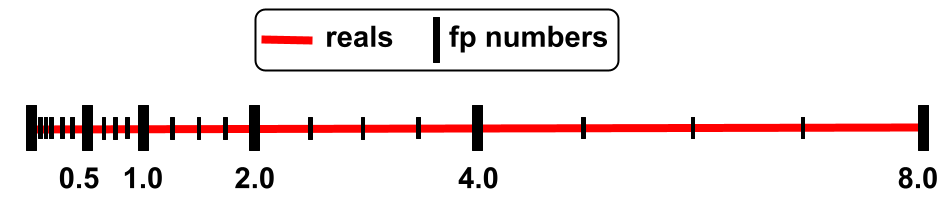
\includegraphics[width=1.0\textwidth]{pic/fpnumbers.png}
	\end{tabular}
	\caption{The spacing between floating-point numbers (black-and-white squares), plotted on the top of the real line (red), is uniform only within two consecutive powers of two.}
	\label{fig:line}
\end{figure}
%
\begin{figure}[tb!]
	\centering
	\begin{tabular}{l}
		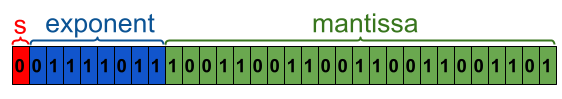
\includegraphics[width=1.0\textwidth]{pic/examplenumber.png}
	\end{tabular}
	\caption{Single precision floating-point representation of the decimal value 0.1 using the default rounding mode round-to-nearest.}
	\label{fig:zeropointone}
\end{figure}
%

Assuming the computation does not overflow or underflow, the standard model of arithmetic~\cite{every} states
%
\begin{align}
fp(x)=x(1+\delta)\;\;\;\text{where}\;\;\;|\delta|\leq\epsilon
\label{standard}
\end{align}
%

where $fp(x)$ is the floating-point value of the real computation $x$, and the error $\delta$ is bounded by the so-called \emph{machine epsilon}, that is the upper-bound on the relative error.
%
The value of \emph{machine epsilon} is format dependent.
%
For example, for single-precision $\epsilon=2^{-24}$, while for double-precision $\epsilon=2^{-53}$.
%
The standard model holds for normal numbers, which are the focus of this thesis.
%

In Figure~\ref{fig:zeropointone}, we report the format representation when the decimal value 0.1 is stored in a single precision (32bits) floating-point variable.
%
The decimal value $0.1$ becomes $0.0\overline{0011}$ in binary, which in normalized form is $1.1\overline{0011}*2^{\text{-}4}$.
%
This number is periodic, and thus it is not exactly representable in single - or any other finite - precision format.
%

Let us discuss the details of the format representation.
%
The sign is zero because the number is positive.
%
The stored value for the exponent corresponds to the decimal 123, on the other hand, we saw the actual value should be -4.
%
This is because the stored exponent is shifted, with respect to the actual value, by the exponent bias. 
%
Thanks to the bias, the exponent is stored as unsigned number, as opposed to signed number, which makes easier an eventual comparison with other floating-point numbers in the future.
%
The bias is computed as $2^{e\text{-}1}\text{-}1$, where $e$ is the number of bits for the exponent representation, and then, it is added to the actual value of the exponent.
%
Thus, if we go back to our example, we have $\text{-}4+(2^{8\text{-}1})\text{-}1=123$.
%

Finally, the last part of the format is for the mantissa representation. 
%
For normal numbers, like 0.1 in our example, the IEEE standard assumes there is always an implicit leading bit, set to one, which is not actually stored in the representation.
%
%In other words, the actual value of the mantissa is obtained by placing a leading 1$1.$\emph{mantissa}.
%
This is called the hidden or implicit bit.

%
The actual value stored in single precision is $0.100000001490116119384765625$ which lead to a roundoff error of approximately $1.49e\text{-}9$.
%

The same number 0.1 evaluated in double precision is stored as \\ $0.1000000000000000055511151231257827021181583404541015625$ with a roundoff error of approximately $5.55e\text{-}18$.
%
\section{Roundoff Error Analysis}
%
The goal of roundoff error analysis is to measure the roundoff error stemming from the floating-point implementation of a program.
%
As we saw in the Patriot Missile catastrophe, roundoff errors are very small, but they propagate through computations and they can rapidly accumulate.
%
%The goal of roundoff error analysis is to measure the approximation errors stemming from the floating-point implementation of a program.
%
%In this thesis, we focus on a so called rigorous (i.e. sound) roundoff error analysis. 
%

The approach we used to measure the rounding error in the program in Figure~\ref{fig:while}, assumes we have a reference implementation to compare with, in the literature often called the \emph{oracle}~\cite{blame}, holding the ideal value of the computation.
%
%In the program, the oracle is the integer variable t.
% 
%In our small example, regardless of its simplicity, shows a critical (and limiting) assumption we are making here, to 

In real-world applications, typically the oracle is not part of the program itself, but rather, it has to be created by the developer as a separate entity.
%
Indeed, the oracle is an exact copy of the original program, where all the floating-point variables (e.g., single or double) have been replace by custom multiple-precision floating-point variables~\cite{mpfr}.
%
In the latter, the developer can specify the bit width of the format for each variable (e.g., 1000bits) and use this high-precision program as a proxy for the ideal (infinite precision) implementation.
%
At this point, we have two copies of the same program, one is the implementation, and the other one is the oracle. 
%
The idea is to run both the implementation and the oracle with the same input values, and ultimately compute the arithmetic difference between the two outputs. 
%
This is going to be the forward roundoff error of the program. 
%

While the oracle based approach has been used in several tools~\cite{landau2014guide, kahan1996improbability, atomic, blame, herbie}, it suffers from several limitations.
%
As we already mentioned, when we use a finite number of bits to perform arithmetic, we commit a roundoff error \emph{regardless} of the bit width of the format.
%
%In other words, using arbitrary wide precision formats (e.g., 1000bits), do not match exactly real arithmetic.
%
Moreover, implementing a high quality high-precision oracle requires much expertise, and thus is expensive in terms of development cost~\cite{atomic}.
%
Finally, using Monte Carlo sampling to exhaustively search the input space results in non-rigorous (i.e. unsound) error bounds~\cite{glasserman2013monte, parker2000monte}.
%

In this thesis, we focus on rigorous (i.e. sound) roundoff error analysis.
%
We give a sound (or rigorous) guarantee if there is 100\% certainty about the guarantee.
%
%Clearly, any approach making probabilistic statements based on Monte-Carlo sampling is unsound.
%
For example, when we say 95\% of the computations obey a certain roundoff error bound $\epsilon$, we are making a sound statement based on some analytical model of the computations, and there is therefore no uncertainty about this statement.
%
%\subsection{Bounding Roundoff Errors}
%
%Interval arithmetic 
%Affine Arithmetic
\subsection{Worst-Case Error Analysis}
\label{sec:worst}
%
A special case of rigorous roundoff error analysis is the so called \emph{worst-case} error analysis, which implies the roundoff error bound holds for any input value.
%

Intuitively, in worst-case analysis we assume the error $\delta$ in Equation (\ref{standard}) has the worst magnitude possible. In other words, we make a conservative choice by setting $\delta=\epsilon$.
%
Clearly, this conservativeness makes our analysis rigorous in the sense there cannot be any outliers.
%

In the last decade, many successful techniques have been used to implement worst-case error analysis~\cite{darulova2018daisy,2015_fm_sjrg,solovyev2018rigorous,rosa,fptuner,smartfloat,satire,gappa,fluctuat}.
%
%Here, the keyword \emph{worst-case} stands for the property of the error bound to hold for \emph{any} input value.
%
The soundness of worst-case error bounds is precious for all those applications, like safety-critical ones~\cite{guardstable, cpralg}, where from the context, we can sense the need to bound the error of any possible computation, included corner-cases or very rare outliers.
%
Intuitively, no one would feel comfortable traveling with autonomous flying aircrafts which are safe \emph{on average}.

%
From an implementation perspective, the main advantage of worst-case analysis is we only need to know the range of the inputs, rather than how the inputs are distributed in such ranges. 
%
Indeed, the resulting error bounds hold for any input value, regardless of the distribution.
%
%This is why the state-of-the-art refers to this non-deterministic model as \emph{worst-case}, because it does not account for the distribution of the inputs.
%
This property is priceless, in particular, when the input distributions are unknown.
%

On the other hand, in Section \ref{sec:prob}, we discuss how \emph{ignoring} the distribution of the inputs becomes a limitation when \emph{we do know} how the inputs are distributed.
%

Finally, a strict requirement of worst-case analysis is the input variables must be bounded  in a finite range. This is because, in the worst-case, unbounded variables lead to unbounded roundoff errors, which in practice, are of little use from an implementation perspective.
%
\section{Thesis Statement}
%
Our thesis statement is the following: 

%
\emph{
%The usability of rigorous roundoff error analysis is minimal in real-world scenarios.
%in practise
%
%Out of the many existing analyzers, only few of them have primordial support for common programming constructs, like conditional statements, while none of them can deal with unbounded input variables nor probability distributions.
%	
In this thesis, we combine rigorous roundoff error analysis and symbolic execution to precisely reason about control-flow instabilities in computer programs.
%
%We use this resulting prototype to verify real-word applications, specifically micro-controllers, and safety-critical software in self-flying aircrafts. 
%
Moreover, we tackle the limitations of worst-case roundoff error analysis, that is to say dealing with probability distributions and unbounded input variables, by introducing our probabilistic framework to compute average roundoff errors as opposed to the state-of-the-art worst-case roundoff errors.
%
%, thus transitioning from worst-case roundoff errors to average roundoff errors.
%
%This allows us to quantify very precisely the idea of probabilistic reliability of the low-precision program.
%
\\
In the next section, I describe what my contributions are.
}

%\emph{\\\\In this thesis we show how to improve the stability of computer programs by encoding the mix of real and floating-point formulas in SMT solvers.
%
%Moreover, in case a developer is willing to trade the accuracy of a computer program for the sake of the efficiency, we can quantify very precisely the idea of probabilistic reliability of the low-precision program.}
%
%the usability of wc error tools in practise is minimal, no conditionals, no probability distributions, no etc. very few established uses scenarios. 
%.. my thesis tackle these problems by combining worst-case analysis with smt (CHAPTER 1 AND 3) solving and probabilistic reasoning as well as applying it in realistic novel uses scenario like the EMSOFT IS THE PRIMARY EXAMPLE OF APPLICATION, OR THE GPS, NASA AIRTRAFFIC CONTROL.
%
%
\section{Contributions}
%
This thesis present techniques for rigorous numerical analysis of computer programs, with several case studies on real-world applications.
%
%The usability of rigorous roundoff error analysis is minimal in real-world scenarios.
%
%Out of the many existing techniques , only few of them have primordial support for common programming constructs, like conditional statements, while none of them can deal with unbounded input variables nor probability distributions.
%
In the next sections, we introduce one-by-one each of the contributions included in this dissertation.
%

In particular, in the next Section~\ref{conditionals} we show, with the help of an example, the need to precisely reason about roundoff errors in conditional statements, as opposed to the conservative approach used in the state-of-the-art.
%

In Section~\ref{controllers}, we discuss how we embedded roundoff error analysis in the design process of Model Predictive Controllers (MPC).
%

Finally, in Section~\ref{sec:prob} we show, with the help of a small example, the limitations of worst-case error analysis and we discuss the need for average roundoff errors as opposed to the state-of-the-art worst-case roundoff errors.
%
%in practise
%
%Out of the many existing analyzers, only few of them have primordial support for common programming constructs, like conditional statements, while none of them can deal with unbounded input variables nor probability distributions.

%In this section, we provide a 
%describe how we tackled the limitations 
%In Chapter \ref{sec:fprock}, we describe FPRoCK (Floating-Point Real Checker), a prototype of an SMT solver we developed to reason about the mix of floating-point and real arithmetics, which is critical to spot instability jumps in computer programs.
%
%We use this resulting prototype to verify real-word applications, specifically micro-controllers, and safety-critical software in self-flying aircrafts. 
%
%Moreover, this thesis tackles the limitations of worst-case error analysis, that is to say dealing with probability distributions with infinite supports, by introducing our probabilistic framework to compute average roundoff errors as opposed to the state-of-the-art worst-case errors.
%
%, thus transitioning from worst-case roundoff errors to average roundoff errors.
%
%This allows us to quantify very precisely the idea of probabilistic reliability of the low-precision program.
%

%\emph{\\\\In this thesis we show how to improve the stability of computer programs by encoding the mix of real and floating-point formulas in SMT solvers.
%
%Moreover, in case a developer is willing to trade the accuracy of a computer program for the sake of the efficiency, we can quantify very precisely the idea of probabilistic reliability of the low-precision program.}
%
%the usability of wc error tools in practise is minimal, no conditionals, no probability distributions, no etc. very few established uses scenarios. 
%.. my thesis tackle these problems by combining worst-case analysis with smt (CHAPTER 1 AND 3) solving and probabilistic reasoning as well as applying it in realistic novel uses scenario like the EMSOFT IS THE PRIMARY EXAMPLE OF APPLICATION, OR THE GPS, NASA AIRTRAFFIC CONTROL.
%

%
%In Chapter \ref{sec:fprock}, we describe FPRoCK (Floating-Point Real Checker), a prototype of an SMT solver we developed to reason about the mix of floating-point and real arithmetics, which is critical to spot instability jumps in computer programs.

%
%In the last decade, there has been a massive usage of low precision implementations (e.g. in artificial intelligence with CNN) primarily to conserve resources such as energy, memory footprint and execution time~\cite{lutnet}.
%
%Clearly, the high demand of resources from floating-point arithmetic is problematic, in particular, when dealing with portable devices (e.g. smart-watches) where the usage and the duration of the battery is a primary concern.
%
%Thus, the need to sacrifice the accuracy of computations in favor of the efficiency.
%
%In Chapter \ref{sec:emsoft}, we describe our framework to design low precision micro-controllers, and we show how we can use static analysis to guarantee the stability of the micro-controller is not affected by the low-precision format.
%
%Indeed, our goal is to guarantee the use of low-precision arithmetic does not impact the reliability of the system.

%
%InWe can use a similar argument to describe the nature of worst-case analysis. 
%

%The current state-of-the-art for roundoff error analysis have primary focused on worst-case error bounds~\cite{darulova2018daisy,2015_fm_sjrg,solovyev2018rigorous,rosa}.
%
%With the keyword \texttt{worst-case} we mean the property of the error bound to hold for \texttt{any} input value.
%
%While this is priceless in, for example, safety-critical applications~\cite{cpr}, there are a variety of (non-safety) applications where a developer might want to trade some accuracy in favor of a lower-cost precision format.
%
%In Chapter \ref{sec:cav}, we describe our probabilistic error analysis, evolving from worst-case analysis, where the developer can set a custom confidence interval of interest (e.g. 85\%, 95\%, 99\%, etc.) and ignore extremely unlikely corner cases, and ultimately obtain more optimal results.
%Worst-case errors and 100\% confidence interval are synonyms.
%
\subsection{Handling Conditionals}
\label{conditionals}
%
While roundoff error analysis has been successfully used to bound straight-line expressions, less attention has been given to other common programming constructs, like conditionals.
%
In this section we describe how the state-of-the-art for rigorous roundoff error analysis handle conditional statements~\cite{precisa, fluctuat} and what are the limitations of their approach.
%

In numerical analysis, it is critical to deal with conditionals because the control-flow of a computer program evaluated in floating-point arithmetic might differ from the ideal flow in real arithmetic.
%
%For example, the condition of an if-statements evaluates to true in real arithmetic, but because of finite-precision arithmetic, the same condition evaluates to false.
%
This is a so called \emph{instability jump}~\cite{satire} or \emph{control-flow instability}~\cite{unstable}.
%
The absolute error stemming from instabilities can be measured as the arithmetic difference between the expressions in the \emph{then} and the \emph{else} branches.
%
%In general, while the roundoff error of straight line expressions is in the order of \emph{machine epsilon}, an instability jump can be in the order of the units, which typically is many orders of magnitude wider than the former.
%

Consider the if-statement reported in Figure~\ref{fig:ifstatement}, 
%
\begin{figure}[tb!]
	\begin{lstlisting}[frame=single, language=Python, escapeinside={(*}{*)}]
	x(*$\;\in\;$*)[0,10]
	if x>5:
	  return 10
	else:
	  return -10	
	\end{lstlisting}
	\caption{A simple if-statement we use to study instabilities.}\label{fig:ifstatement}
\end{figure}
%
where we have the variable \emph{x}, bounded in the interval [0, 10], flowing into the condition of an if-statement.
%The \emph{then} branch returns $10$, while the else branch returns $-10$.
%

\begin{figure}[tb!]
	\centering
	\begin{tabular}{ll}
		
\includegraphics[width=0.5\textwidth]{pic/ifreal.png}
		&
		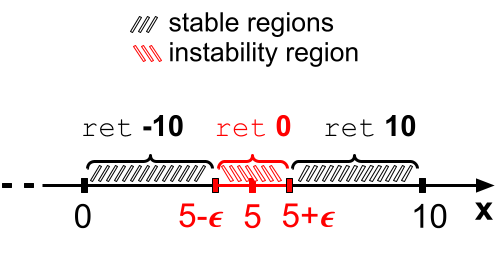
\includegraphics[width=0.5\textwidth]{pic/iffp.png}
	\end{tabular}
	\caption{The evaluation of a simple if-statement in case of real arithmetic (left) and the floating-point counterpart (right). In red you can see the instability region, where $\epsilon$ is the roundoff error accumulated by the variable X.}
	\label{fig:ifreal}
\end{figure}

In Figure \ref{fig:ifreal}, we plot the instability region for our if-statement. Clearly, when we compute in real arithmetic we do not have instabilities. On the other hand, in floating-point computations, we can identify the \emph{instability region} as that part of the input domain from where instabilities might be triggered.
%
The width of the instability region is determined by the roundoff error $\epsilon$, and in our example, $\epsilon$ is the roundoff error accumulated by $x$. From Equation (\ref{standard}), we know the roundoff error is proportional to $x*(2^{-p})$ where p is the bit-width of the floating-point format, and assumes maximal magnitude when $x=10$.  
%
In double precision floating-point arithmetic (64-bits), $\epsilon$ equals $1.11e^{-15}$.
%
By using $\epsilon$ we can modify our program and make it \emph{robust} to roundoff error.
%
\begin{figure}[tb!]
	\begin{lstlisting}[frame=single, language=Python, escapeinside={(*}{*)}]
	x(*$\;\in\;$*)[0,10]
	if x>5+(*$\epsilon$*):
	  return 10
	elif x<(*$5-\epsilon$*):
	  return -10
	else: #we landed in the instability region
	  return 0
	\end{lstlisting}
	\caption{A \emph{robust} if-statement where the real execution and the floating-point counterpart always coincide.}\label{fig:ifrobust}
\end{figure}
%

In Figure~\ref{fig:ifrobust} we report the robust program, where the ideal and the floating-point executions always coincide. 
%
In other words, when the real execution returns the value 10 also the floating-point counterpart returns 10. Similar argument holds for the return value -10.
%
Clearly, in the robust program, we need to consider the case we land in the instability region. Thus, we make the arbitrary decision to return the value $0$ to handle this situation.

%On the other hand, the instability jump can be computed (statically) as $|10-(-10)|=20$. There are about 16 orders of magnitude between the roundoff error and the instability jump error.
%

Let us now slightly modify the range of the input variable x in our example. 
%
In particular, we set the range of x to the closed interval $[0, 10^{300}]$, and with the same reasoning used so far, we compute the new width of the instability region and we get $\epsilon=7.43e^{283}$.
%

This new size for the instability region is almost as wide as the max-representable value in double-precision, and of little use from an implementation perspective. 
%
Clearly, with this new value for $\epsilon$, the approach used so far to make the program \emph{robust} to roundoff errors, is extremely conservative from an implementation perspective, because almost all the computations, both the stable and the unstable ones, are going to land in the instability region.
%
Moreover, the return value -10 becomes unreachable, meaning the robust program is never going to return -10, which is also of little use from an implementation perspective.
%
%Assuming \emph{any} computation landing in the instability region leads to an instability jump is of little use from an implementation perspective.
%

This shows how critical it is to precisely reason about roundoff errors in conditionals.
%
\subsection{Application to Controller Synthesis}
\label{controllers}
%
Floating-point numerical algorithms are essential to many applications and it is often desirable to compute their results as accurately as possible.
%
Control system designers using existing toolboxes, for example in MATLAB, use the well-known floating-point formats, single and double, as a proxy for real (ideal) arithmetic. 
%
Indeed, at design time, the main concerns are closed-loop performance and the stability of the system.
%

%In the design of controller applications for embedded systems there is the need to take particular care for roundoff errors stemming from finite precision computations.
%
%Finite-precision numbers induce roundoff errors, and knowledge of the range of these roundoff errors is required to fulfill safety criteria of critical programs, as typically arising in modern embedded systems such as aircraft controllers.
%
On the other hand, from an implementation perspective, meaning when it is time to deploy the controller on the chip, other factors such as performances, hardware dimensions, and energy consumptions become primary concerns~\cite{suardi}.
%
In the last decade, there has been massive usage of low precision floating-point formats, for example in artificial intelligence (AI), with the aim of conserve resources~\cite{fppower}.
%
Hence, leveraging low precisions can lead to significant savings, and the impact of low-cost floating-point precisions on machine learning predictors is an active research area.
%
The main drawback is that low precision arithmetics imply a greater tolerance towards implementation errors.
%

The natural question then would be whether we can \emph{implement} the \emph{ideal} controller (from MATLAB) using low-precision formats, while still guarantee the stability of the system.
%
In other words, in case we implement a controller using low-precision formats, would the controller still be able to govern the system for which it has been designed for.
%

In our framework, we embed the state-of-the-art for worst-case error analysis in the design of linear time invariant Model Predictive Controllers (MPC).
%
In our approach, the roundoff error stemming from the finite-precision implementation of the controller is measured using static-analysis, and then embedded in the set of all the disturbances affecting the system.
%
Typically, a controller is designed to handle various sources of external disturbances, like for example, friction or wind resistance.
%
At design time, the designer of the controller estimates the total disturbance $\Delta$ the controller has to tolerate.
%
Since $\Delta$ accounts for any source of disturbance affecting the system, it is also called the "disturbance budget".
%
Our idea consists in including the roundoff error stemming from the finite-precision implementation of the controller as an additional disturbance affecting the system.
%
Thus, our is an iterative based approach, where we reduce the bit-width for the arithmetic and the memory foot-print of the controller, until the roundoff error violates the budget delta.
%
This is going to be the minimal lowest-cost controller which does not violate the budget delta, and thus the stability of the system is not affected.
%
%Furthermore, we use the so called mixed-precision tuning to further reduce the precision of the co, using the assumption that there might be only certain area that have to be computed precisely and not all of them.

%WORST-CASE ANALYSIS HAS NOT BEEN EMBEDDED IN REAL WORLD %APPLICATIONS (LIKE WHAT YOU DID IN EMSOFT).
%
%  
%  
%
%WE WANT TO HELP DEVELOPERS.
%
%LIMITATIONS OF WORST CASE ANALYSIS IN CASE OF DISTRIBUTION.
%
%
\subsection{Probabilistic Error Analysis}
\label{sec:prob}
%
In this section, we describe what are the limitations of worst-case roundoff error analysis, and we introduce our framework to compute probabilistic (or conditional) roundoff error bounds.
%
As we mentioned earlier, worst-case analysis could provide conservative error bounds in case we know \emph{a priori} the distribution of the inputs. 
%
%Furthermore, we must bound the input variables to prevent overflow and thus unbounded roundoff errors.
%

In our probabilistic framework, we use probabilistic range analysis to compute conditional roundoff errors where, as opposed to the worst-case approach, the roundoff error is computed with respect to the computation landing in a given confidence interval of interest (e.g., 85\%,99\%, 99.9999\%).
%
Note, in the worst-case approach, there is an implicit 100\% confidence interval, thus worst-case analysis and 100\% confidence interval are synonyms.
%

%
Let us discuss the limitations of worst-case analysis on the program reported in Figure~\ref{fig:prob}.
%
\begin{figure}[tb!]
	\begin{lstlisting}[frame=single, language=Python]
	if c(x)>constant:
	  return 1/0 #ERROR
	else:
	  return 0 #OK
	\end{lstlisting}
	\caption{A simple if-statement we use to study the conservativeness of worst-case analysis. The \emph{then} branch leads to an error while the \emph{else} branch returns correctly.}
	\label{fig:prob}
\end{figure}
%
We consider \lstinline{c(x)=x}, and we assume the variable $x\sim Normal(0,1)$ is distributed accordingly to a standard normal with parameters $\mu = 0$ and $\sigma = 1$.
%
At line 1, we compare c(x) with a constant value.
%
In case the comparison evaluates to true, the \emph{then} branch leads to an error (division by zero), otherwise, the \emph{else} branch returns correctly.
%

\emph{Regardless} of the value of the constant used for the comparison, \emph{any} rigorous (i.e. sound) worst-case range analysis is going to signal a potential division-by-zero error at line 2.
%
In other words, the worst-case analysis is going to terminate as soon as a potential division by zero is detected.
%
This is because, in case the error at line 2 is triggered the program would crash, and thus, it would not make sense to reason about ranges or roundoff errors.

%
A developer using such worst-case tools has no information about \emph{how rare} might be the condition leading to such crash. 
%

In our probabilistic framework, we know the standard normal distribution concentrates more than 99\% of probability mass in the interval $[−3, 3]$, and less than 0.5\% of mass spreads in the interval $[3, \infty]$.
%
If we go back to our example, in case we set the constant at line 1 equal to 1000, a developer using our combined analysis, might not be interested in the very rare outliers triggering the error at line 2.
%
Thus, we can run our probabilistic analysis with a \emph{confidence interval} set, for example, to 99\%.
%
%Clearly, other confidence intervals of interest could be used. 
%
With this setting, not only the program terminates correctly (return 0), but our conditional error bound for $c(x)=x$ is $\epsilon = 3*(2^{-p})$.
%

In general, by studying the \emph{average} execution of a computer program we can prune away very rare corner cases and provide meaningful directions to the developer.
%
\newpage
\bibliographystyle{plain}
\bibliography{\jobname}

%When we trade the accuracy of a computation for efficiency, what can we say about property of our system like stability or soundness. In alternative, in case we cannot guarantee soundness anymore, can we measure exactly how much unsoundness our application has to be able to tolerate.
%
%This is critical when we want to bound roundoff errors for programs rather than for arithmetic expressions.
%
%We use 
%

%
%Efficiently collecting data and systematically analyzing them is essential to gaining insight into the behavior of complex programs and help developers fix the flaws of the program. Also, given the rich set of concurrency primitives in modern languages, one needs to articulate nuanced concurrency coverage metrics and demonstrate their attainment.
%
%And this is my thesis statement: exact reasoning about roundoff error is hard. We can use exact reasoning for handling conditionals (like we show with FPRock). Overapproximation works for real world problem, like EMSOFT, but it is worst-case. We show how a probabilistic analysis can tackle the limitations of worst-case analyisis in real world applications.